% +--------------------------------------------------------------------+
% | Sample Chapter 3
% +--------------------------------------------------------------------+

\cleardoublepage

% +--------------------------------------------------------------------+
% | Replace "This is Chapter 3" below with the title of your chapter.
% | LaTeX will automatically number the chapters.
% +--------------------------------------------------------------------+

\chapter{Diseño de la aplicación}
\label{makereference3}

\section{Stakeholders}
\label{makereference3.1}

\section{Escenarios}
\label{makereference3.2}

\section{Requisitos funcionales}
\label{makereference3.3}

\section{Interfaz de usuario}
\label{makereference3.4}

\section{Sistema de recomendación}
\label{makereference3.5}

\section{Prototipos}
\label{makereference3.6}

\subsection{ARCore} 
\label{makereference3.6.1} 
 
\subsection{ViroMedia} 
\label{makereference3.6.2} 

\newpage
\subsection{Vuforia + Android} 
\label{makereference3.6.3} 
 
\begin{flushleft}
En este prototipo utilizamos la librería nativa de Vuforia para Android para 
realizar las pruebas de tecnología de reconocimiento de imágenes tanto en  
local como usando la nube que nos ofrecía Vuforia, para la posterior renderización
de objetos y textos.

Las características tecnológicas de este prototipo son las siguientes:
\end{flushleft}

\begin{enumerate}
    \item La librería de Vuforia para android está diseñada a muy baja nivel.
    \item Vuforia para dibujar en 3D usa la librería OpenGL.
    \item OpenGL utiliza una serie de espacios donde se va colocando las cosas: 
    \begin{enumerate}
        \item \textbf{Local space}: Es el espacio local de cada objeto.
        \item \textbf{World space}: Es el mundo donde se encuentra los objetos.
        \item \textbf{View space}: El mundo visto desde la perspectiva de la cámara.
        \item \textbf{Clip space}: Se integra con la pantalla del móvil y definiendo los límites visibles, se establecen unas coordenadas de rango (-1,-1) - (1,1).
    \end{enumerate}
    \begin{flushleft}
        Las transformaciones de estos espacios se realizan mediante matrices 4x4, 
        en las que la primera fila hace referencia a la coordenada x, la segunda a la coordenada y y la 
        tercera a la coordenada z, mientras que la última columna hace referencia a los desplazamientos 
        de los objetos en esos 3 ejes.
        \end{flushleft}
        
            \break
            \break
        
            \begin{figure}
                \centering
                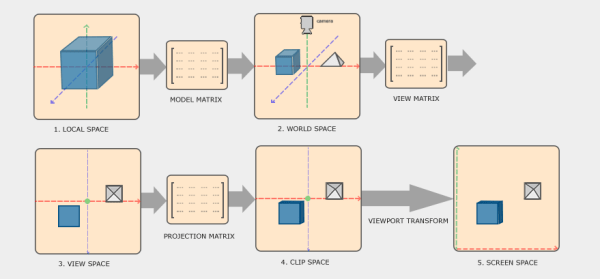
\includegraphics[width=5in]{figures/space-transformation.png}
                \caption{Esquema de los distintos espacios que usa OpenGL}
            \end{figure}
           
            \break
            \break
        
            \begin{figure}
                \centering
                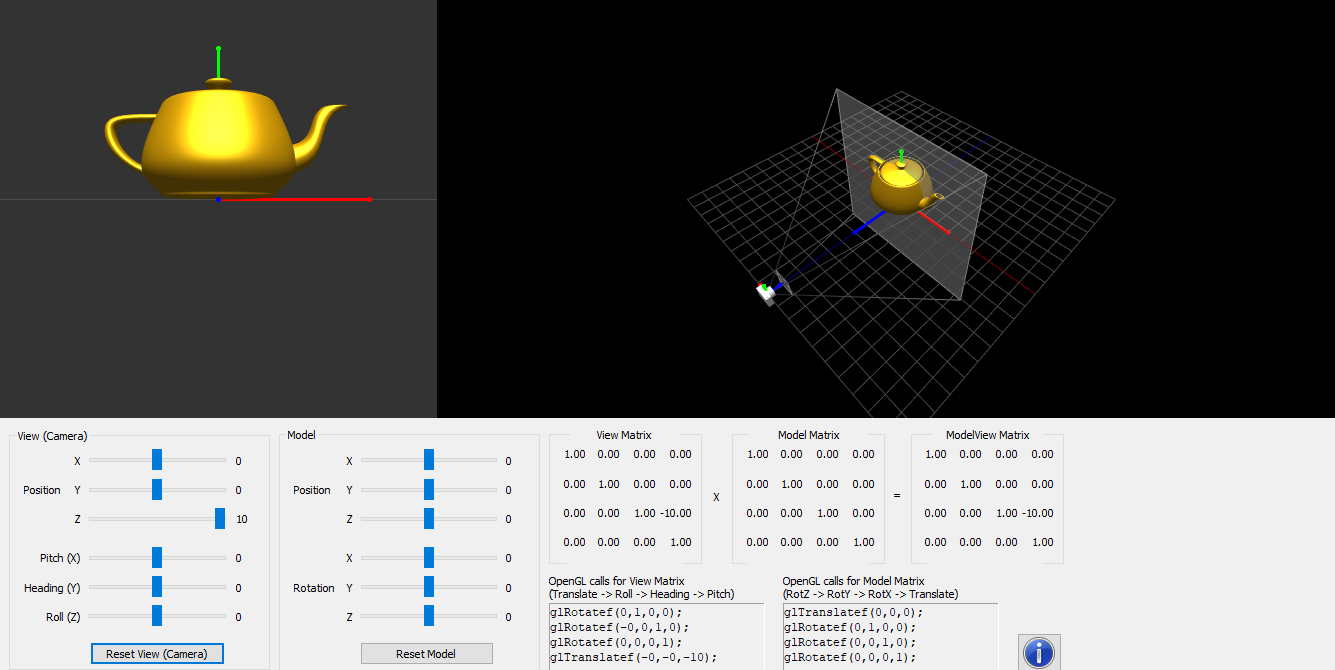
\includegraphics[width=5in]{figures/teapot.png}
                \caption{Ejemplo de un modelo en 3D}
            \end{figure}
    
    \item En OpenGL es necesario escribir código para que las tarjetas gráficas rendericen el modelo 3D,
    el lenguaje que se usa es GLSL. Este código de GLSL se escribe en forma de String y se llama a un método 
    que proporciona OpenGL.
    \begin{figure}
        \centering
        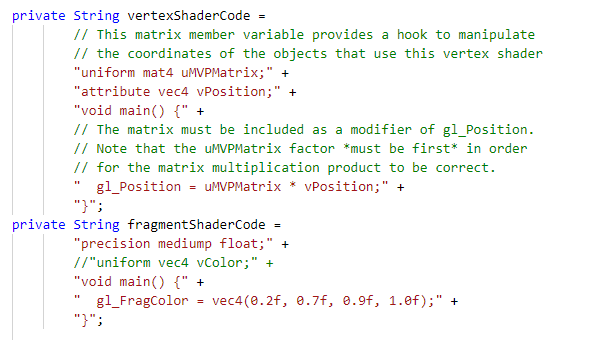
\includegraphics[width=5in]{figures/GLSL.png}
        \caption{Código en GLSL}
    \end{figure}
        
    \item Otro aspecto a tener en cuenta es que OpenGL solo ofrece lo básico, no nos ofrece métodos para dibujar 
    directamente objetos sino que hay que seguir un pipeline de procesos para conseguir dibujar algo.
    \newline
    \begin{flushleft}
    Esto consiste en pasar un array de números (cada tres para definir un punto) 
    a las tarjetas gráficas, establecer triángulos entre los puntos (más arrays de números) 
    definir colores a partir de los puntos (más arrays)..., y con el código del shader, ejecutar 
    estos datos.
    \begin{figure}
        \centering
        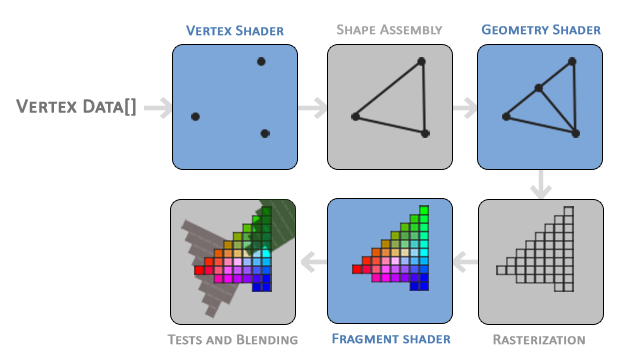
\includegraphics[width=4in]{figures/pipeline.png}
        \caption{Pipeline de la construcción de un modelo}
    \end{figure}
    \end{flushleft}
    \newpage
    \item Por último como sólo ofrece métodos básicos, no hay métodos de escritura de texto, y la forma que 
    encontramos y que funcione fue usar un bitmap con los caracteres. Rechazamos esto por un principal motivo, para hacer que funciones hay que codificar a muy bajo nivel y 
    nos costaría mucho tiempo y esfuerzo.
    \begin{figure}
        \centering
        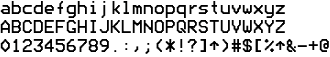
\includegraphics[width=5in]{figures/bitmap-font.png}
        \caption{Mapa de bits de caracteres usado}
    \end{figure}
\end{enumerate}
 

\subsection{Vuforia + Unity} 
\label{makereference3.6.4}